\documentclass{article}
\usepackage[utf8]{inputenc}
\usepackage{graphicx}
\usepackage{subcaption} 
\usepackage{hyperref}

\usepackage[margin=1in]{geometry}

\renewcommand{\familydefault}{\sfdefault}

\title{Stats NZ COVID-19 Wellbeing Indicators }
\author{Vanessa Putnam}
\date{\today} 

\begin{document}
\maketitle

Wellbeing statistics measure how people feel about their lives. Measures do not necessarily include how healthy a person is, but instead measure life satisfaction, finances, health, housing, human rights, and relationships. The following document reports the impact of COVID-19 on New Zealand's wellbeing during the level-4 lockdown peroid 25th March to the 27th of April 2020.

\subsection*{Finances}
Although, finance is commonly associated with the economy, household and personal finances are an important aspects of overall wellbeing. Specifically a Stats NZ analysis found that unemployed people are more likely to rate their overall life satisfaction poorly than employed people or those not in the labour force \href{https://www.stats.govt.nz/news/unemployed-people-less-satisfied-with-life}{[source link]}. The following graphs show that employment as well as income was severely impacted from the COVID 19 lockdown period. 

\begin{center}
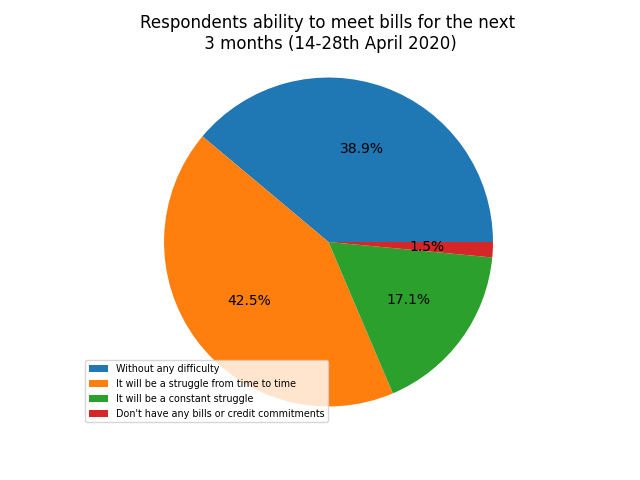
\includegraphics[scale=0.5]{plots/household.png}
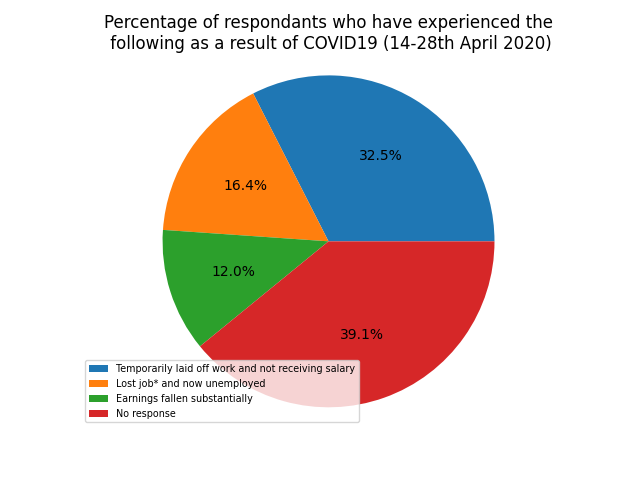
\includegraphics[scale=0.5]{plots/personal.png}
\end{center}

\begin{center}
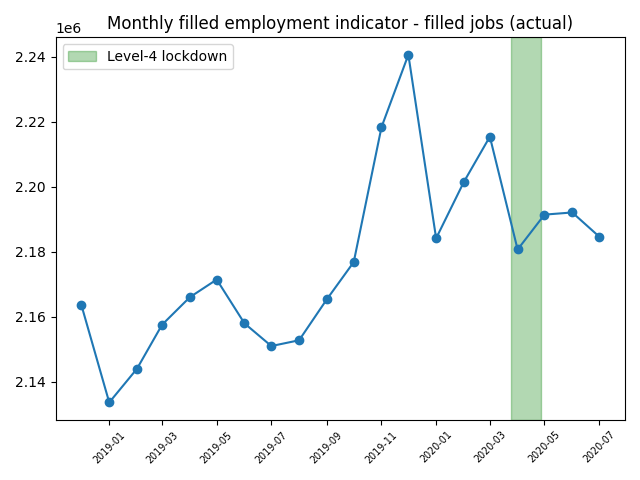
\includegraphics[scale=0.5]{plots/jobs.png}
\end{center}

\vspace{5cm}
\subsection*{Indicators Potentially Effected by Financial Wellbeing}

Although economic sentiment reflects the state of the economy, it is important to note that the negative sentiment during this time also corresponds to a time of major job losses and financial stress. Future work should be done to compare the household and personal fiances as a time series to check if this is a continued reflection of economic sentiment. 

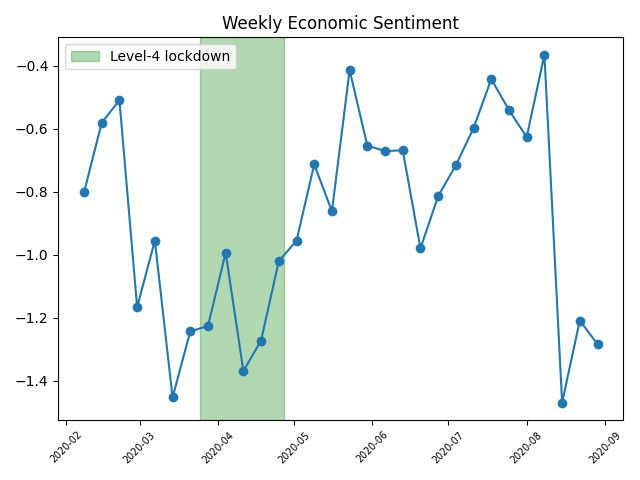
\includegraphics[scale=0.5]{plots/econ.png}

The start of level4 also uncovered various scams. The major job and financial losses could have triggered desperation in people to make ends meet. Future work should be done to compare the time series of personal finances with the increase or decrease in scam related activity. 

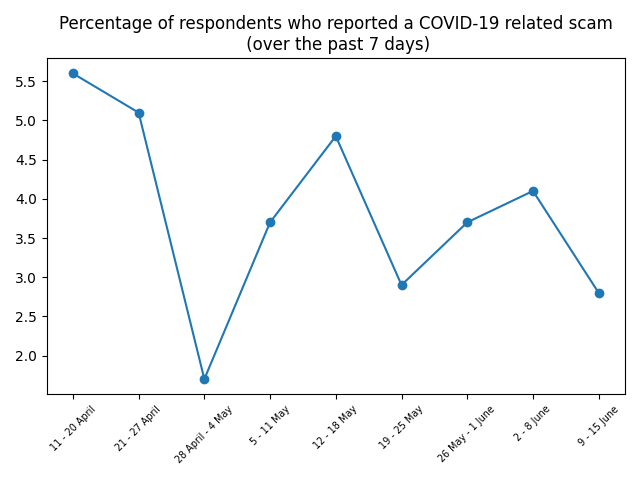
\includegraphics[scale=0.5]{plots/scam.png}

\end{document}
